\documentclass[Main/main.tex]{subfiles}

\begin{document}

 \section{Introduction}

%Define and delimit the problem
%Point out the motivation of the study
%General theoretical background
%Science perspective


This work consists of two parts, exploration of a new liquid injection system for the synthesis of oxides and application of this method to synthesize cathode materials directly on a current collector. These novel cathodes will not need a traditional binder in order for the cathode material to stick to the conducting surface. Thus, cathodes produced by liquid injection may prove to be useful in the future.


Today, we surround ourselves with electricity - from electrical watches and smartphones to electrical cars and light. The aim for a greener future, together with the increasing complexity and finesse of electrical devices calls for a constant development of our device for storing electrical energy - the battery.

Batteries are commonly divided into two categories; primary and secondary batteries. Primary batteries cannot be electrically charged and are therefore single use, whereas secondary batteries are rechargeable. The latter can offer savings in costs and resources. A battery consists of three major parts; the anode, the electrolyte and the cathode. The latter plays an important role when it comes to improving various aspects of batteries, such as cost, safety, power and energy densities \cite{gandrud}. Nowadays, the cathode is typically the most costly element, comprising about 30 \% of the total price of the battery \cite{costcath}. Moreover, as shown in figure \ref{fig:1_discharge_specific} (a) and (b), present cathode materials exhibit around half the specific capacity as the carbon anodes used today \cite{1_rev_liion}.

\begin{figure}[ht]
	\begin{subfigure}[b]{0.5\textwidth}
		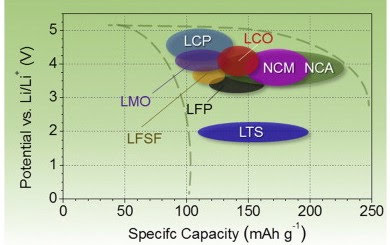
\includegraphics[scale=0.62]{Uploads/1_discharge_specific_cathode}
		\caption{intercalation-type cathodes}
		\label{fig:1_dis_a}
	\end{subfigure}
	~ \quad 
	\begin{subfigure}[b]{0.5\textwidth}		
		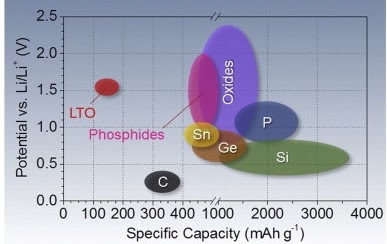
\includegraphics[scale=0.62]{Uploads/1_discharge_specific_anodes}
		\caption{converson-type anodes}
		\label{fig:1_dis_b}
	\end{subfigure}
    \caption{Approximate range of average discharge potentials and specific capacity of some of the most common electrodes in todays researched and commercial batteries \cite{1_rev_liion}.}
    \label{fig:1_discharge_specific}
\end{figure}

\newpage
\subsection{History}

The first electrical battery is credited to the Italian physicist Alessandro Volta who, in 1800, invented the Voltaic pile consisting of alternating disks of zinc and copper separated by brine-soaked paper \cite{1_volta}.\  Since then, a lot of different chemistries and structures have been tested. Among these we find the first rechargeable battery, the Lead-Acid battery, which to present day is being used to start internal combustion engine cars. Later, the alkaline battery used in regular household devices, which are typically non-rechargeable, saw the light of day. \cite{1_yazami}

The next big breakthrough, however, came from Sony Corporation in 1991 with the pairing of a \ce{LiCoO2} (LCO) cathode and a graphite anode to manufacture and commercialize the first mass-produced rechargeable lithium battery \cite{1_hist}. Li-ion batteries had been researched since 1970, starting with fundamental research into intercalation of Li into layered transition-metal sulfides and selenides \cite{Goodenough2013}.
In 1980, John B. Goodenough and his research group found \ce{LiCoO2} to be a stable cathode material capable of donating Li-ions. Later, in 1983, Rachid Yazami was exploring Li intercalation onto graphite and found reversible Li insertion into carbon to avoid a rather pressing problem of dendrite formation, causing the battery to short circuit \cite{1_yazami}. Lastly, Akira Yoshino made use of these discoveries and invented the Li-ion battery as we know it today in 1985. This battery system comprised of a "non-aqueous secondary battery using transition-metal oxides containing lithium ion such as \ce{LiCoO2} as a positive electrode and carbonaceous materials as a negative electrode" *REF*. 


\subsection{The Li-ion battery}

The Li-ion battery (LIB) can be credited for the wireless revolution of portable computers, cell phones and tablets that has revolutionized global communication and is starting to reshape travel as well. As shown by companies such as Tesla, Kia and Nissan, the internal combustion engine can be replaced by a combination of a portable rechargeable battery and an electrochemical capacitor.
There are, however, some imminent questions regarding cost, safety and driving range.  

Li-ion batteries possess certain fundamental advantages compared to other chemistries. Li, being the third element in the peri
Li-ion batteries have an unmatched combination of high power and energy density. This

The batteries assembled and tested for this thesis have consisted of various cathodes manufactured by liquid injection, aiming for \ce{MnO2}, \ce{LiMn2O4} and \ce{LiNi_{0.5}Mn_{1.5}O4}. Moreover, an anode of lithium metal and a liquid electrolyte has been used. 

\subsubsection{Cathodes}
An ideal cathode possess high energy and power densities, is small and inexpensive. Compared to Cobalt, Manganese is a very cheap element, making Mn a potential candidate for cheaper cathode materials. 

A huge variety of cathodes has been researched, including, but not limited to, intercalation cathode materials, transition metal oxides, polyanion compounds and conversion cathode materials. LCO, introduced by Goodenough and commercialized by SONY, is the first and most commercially successful type of layered transition metal oxide cathodes *ref present and future* 

An intercalation cathode contains a solid host network and is able to store guest ions which can be inserted into and removed from the host network reversibly. In a LIB, \ce{Li+} acts as the guest ion while the host network can be metal chalcogenides, polyanion compounds or transition metal oxides. It is common to divide intercalation compounds into crystal structures, such as layered, spinel and olivine.. \cite{1_rev_liion}

\textbf{History of cathodematerials. Especially MnO2, LMO and LNMO}

\paragraph{\ce{MnO2}}


\paragraph{\ce{LiMn2O4} (LMO)}~\\[0.8em]
Spinel \ce{LiMn2O4} has low toxicity, good safety performance and low cost and is thus considered to be an ideal cathode material for LIBs.

\paragraph{\ce{LiMn_{1.5}Ni_{0.5}O4} (LNMO)}~\\[0.8em]
By doping the spinel LMO with a certain amount of transition metal elements, for instance Ni, the Fermi energies of the material can be adjusted and their electrode potentials increased as desired *rewrite and ref - LNMO paper*

Among doped spinel cathode materials, \ce{LiMn_{1.5}Ni_{0.5}O4} (LNMO) has proved promising in terms of performance and discharge capacity. *Talk about charge-discharge platform?

\subsection{Prior work}

To the authors knowledge, there has not been any extensive research into synthesising oxides using liqui injection. There has, however been a lot of research into batteries and cathode materials. 

\subsubsection{Spray pyrolysis}
Spray pyrolysis is an aerosol process that atomizes a solution and heats the droplets to produce solid particles
- Cerpotech

\textbf{Detail into \ce{MnO2}, LMO and LNMO?
What to put under "history" and what to put here?}

\todo[inline]{Explain how oxides for batteries "typically" are made}

What has been done with liquid injection previously?


Something about binders?


%Sem tech Spray pyrolyse - liquid injection er et alternativ
%Hvordan fremstille katodematerialer? Hva gjøres i dag?


\subsection{Definition of the thesis}

Explore the novel method of liquid injection \textit{in vacco} and test out different parameters. Next, use this method to synthesize oxides directly on conducting steel plates and build batteries.





\end{document}